\documentclass[serif]{article}

\usepackage{graphicx}
%\usepackage[brazil, english]{babel}
\usepackage{mathrsfs,amssymb,amsmath,enumerate}
%\usepackage{tgschola}
\usepackage{verbatim,graphicx,geometry,color}
\usepackage{caption, subcaption}
\usepackage[utf8]{inputenc}
%\usepackage{setspace}
\usepackage{amsthm}

\newtheorem{prop}{Proposition}
%\newtheorem{lemma}{Lemma}[section]
\theoremstyle{definition}


\newcommand{\E}{\mathbb{E}}
\newcommand{\Var}{\mathrm{Var}}
\newcommand{\plim}{\overset{p}{\longrightarrow}}
\newcommand{\dlim}{\overset{d}{\longrightarrow}}

\usepackage{hyperref}
%\hypersetup{
%  colorlinks = true,
%  linkcolor = red!60!black,
%}
%\renewcommand{\thefootnote}{\arabic{footnote}}
%
%\makeatletter
%\let\@mycite\@cite
%\def\@cite#1#2{{\hypersetup{linkcolor=blue!60!black}[{#1\if@tempswa , #2\fi}]}}
%\makeatother


\begin{document}


\begin{itemize}
\item The value of the subsidies considered were: 2, 5, 10, 20 and 30\% for both new technologies or new combinations. We could do more, but the simulations tend to take longer when subsidies are higher.
\item The subsidy runs for 30 years, starting in 2016 (180 years after the simulations starts).
\item I ran 20 simulations of the model. 
\end{itemize}

\begin{figure}[h!]
\begin{subfigure}[b]{0.45\textwidth}
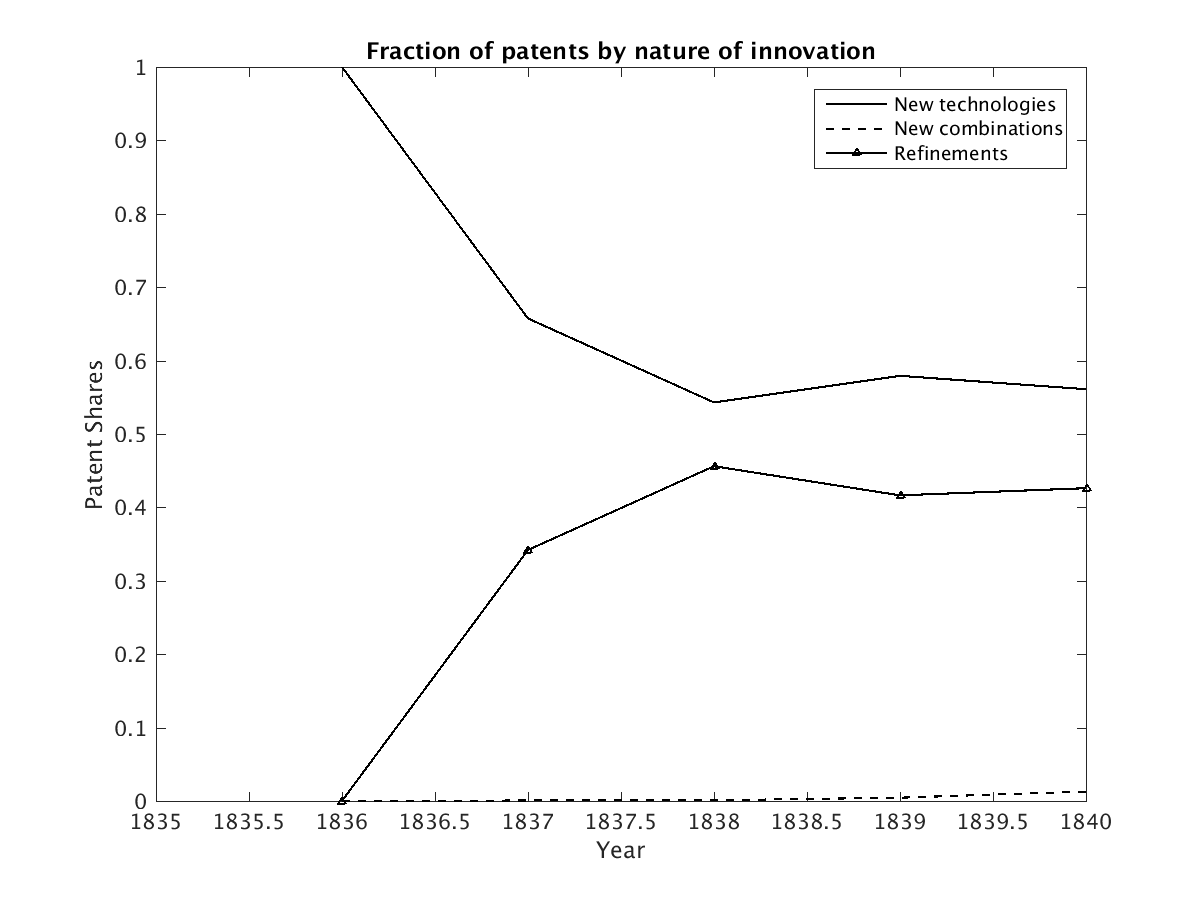
\includegraphics[width=\textwidth]{figures/patents.png}
\subcaption{Model.}
\end{subfigure}
\begin{subfigure}[b]{0.45\textwidth}
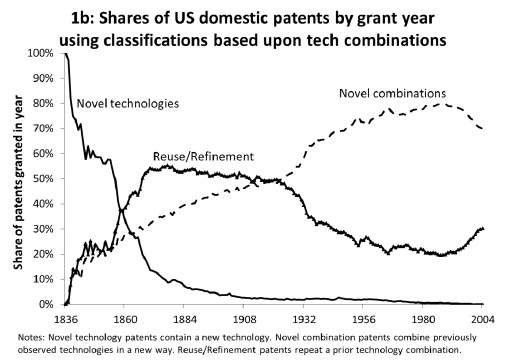
\includegraphics[width=\textwidth]{figures/patents_data.png}
\subcaption{Data.}
\end{subfigure}
\end{figure}

\begin{figure}[h!]
\centering
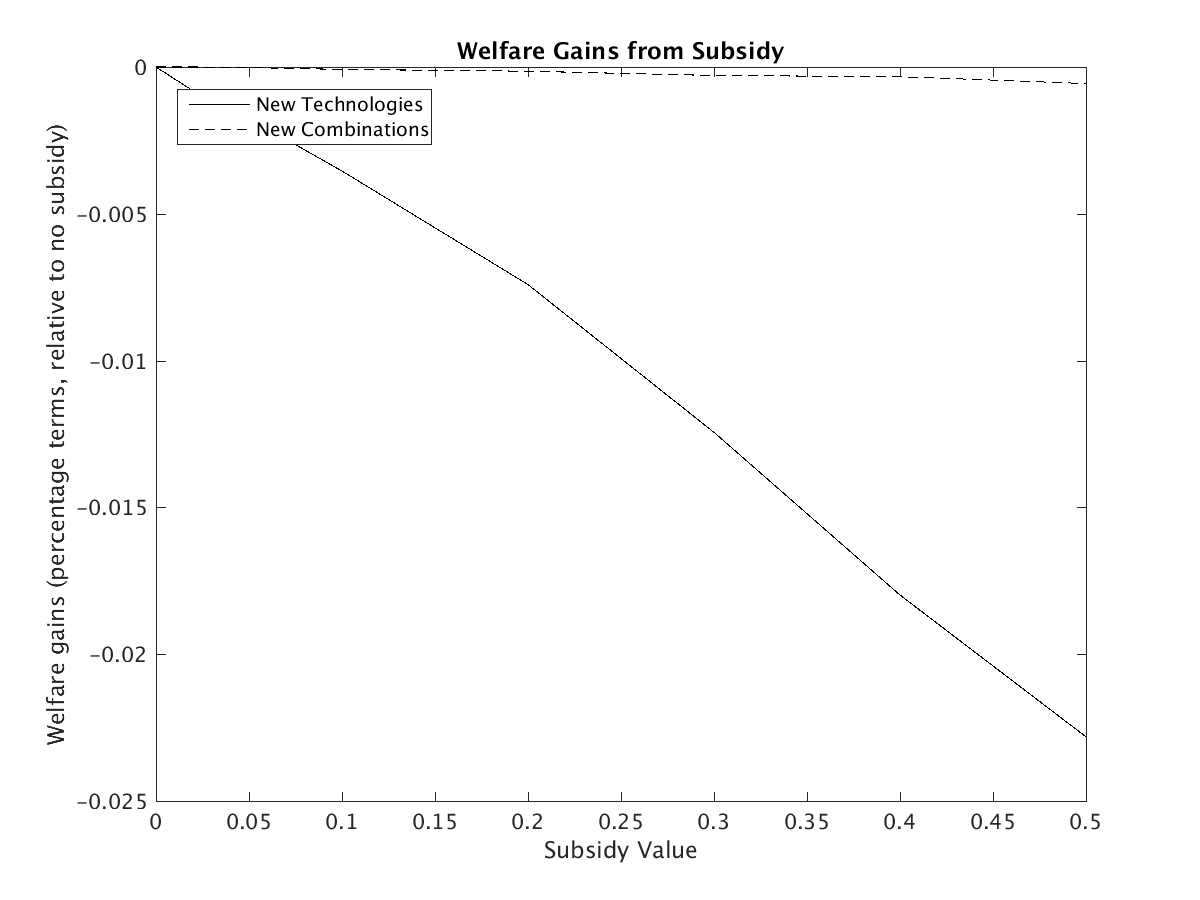
\includegraphics[width=.8\textwidth]{figures/welfare_gains.png}
\end{figure}

\clearpage

\section*{Other Figures}

\begin{figure}[h!]
\centering
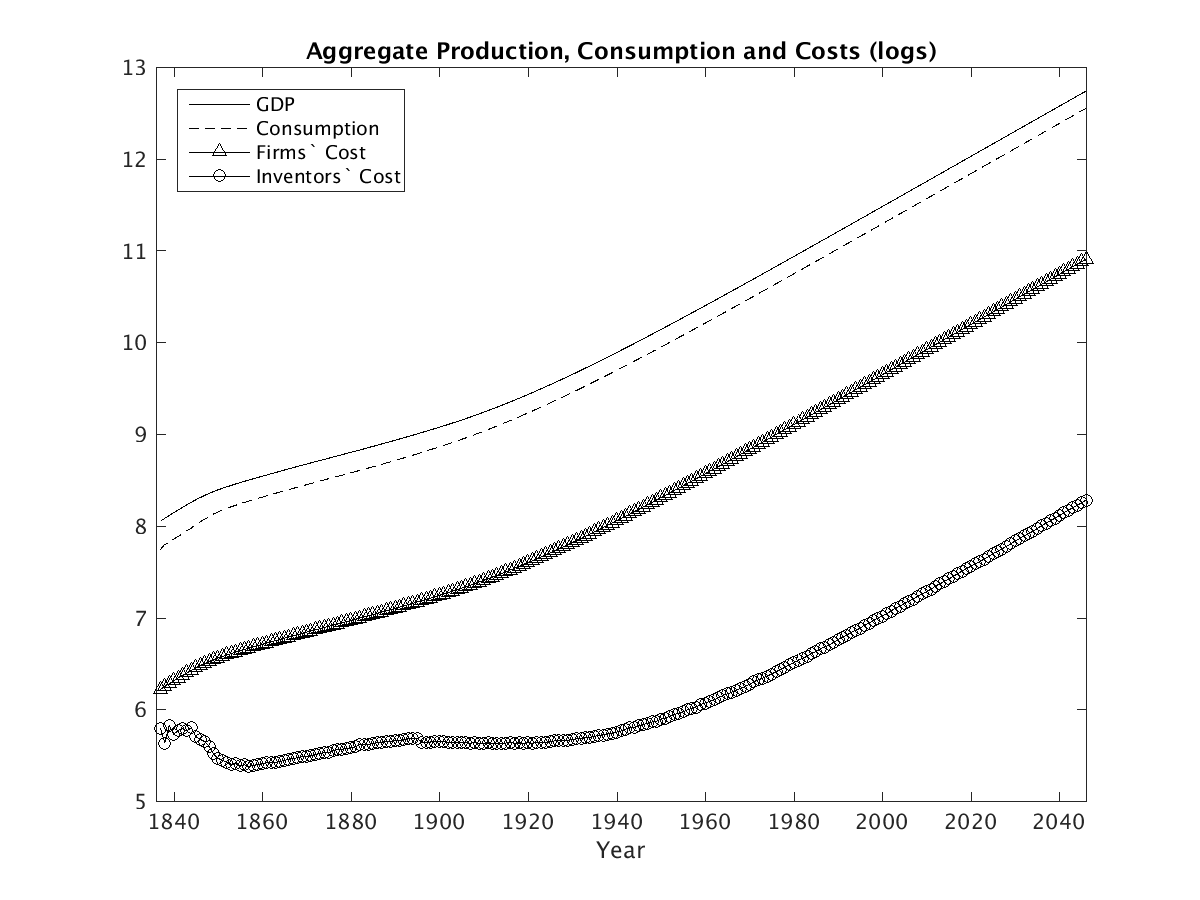
\includegraphics[width=\textwidth]{figures/aggregates.png}
\caption{Value of aggregate variables in the economy.}
\end{figure}

\begin{figure}[h!]
\centering
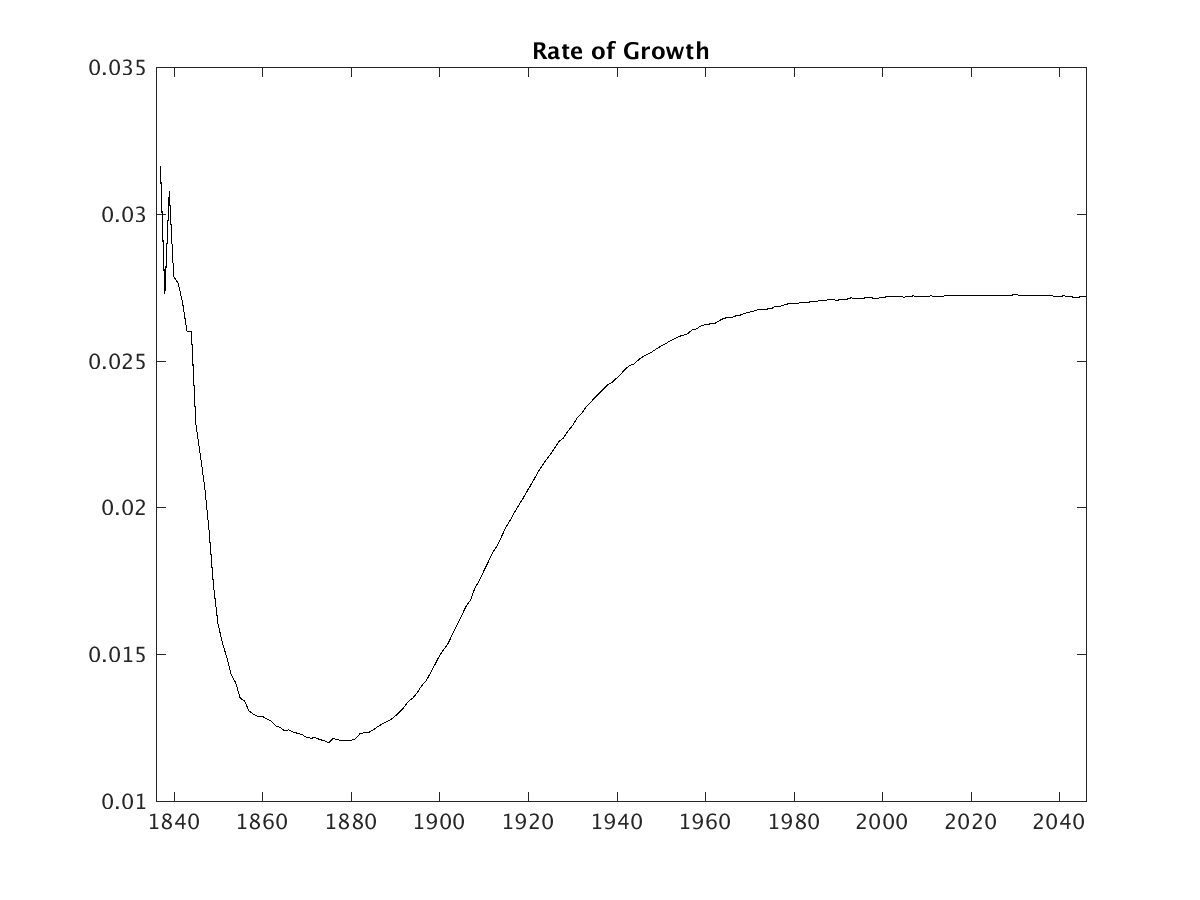
\includegraphics[width=.75\textwidth]{figures/growth.png}
\caption{Evolution of the rate of growth.}
\end{figure}

\begin{figure}[h!]
\centering
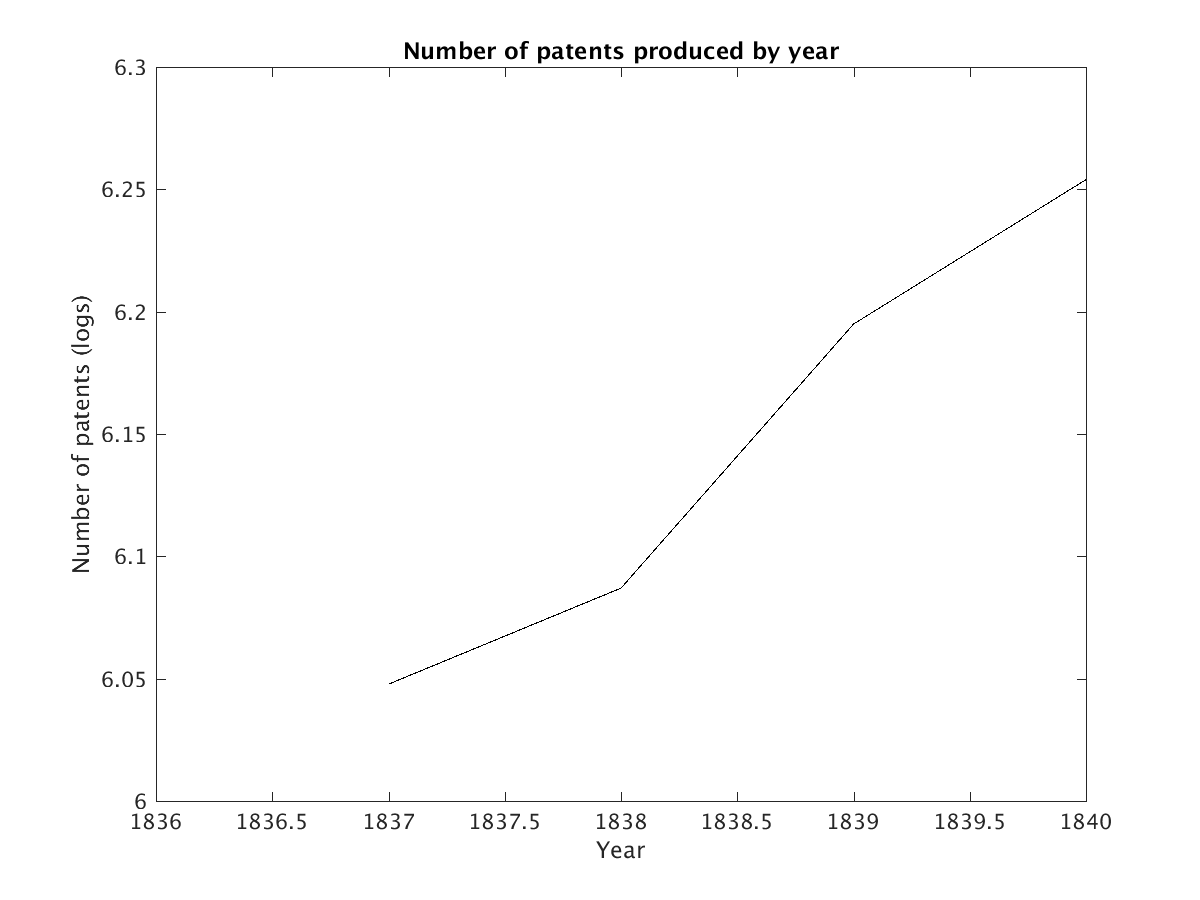
\includegraphics[width=.75\textwidth]{figures/num_pats.png}
\caption{Number of patents produced each period.}
\end{figure}


\end{document}